\documentclass[]{article} 
\usepackage{proceed2e}

\usepackage[numbers,sort]{natbib}
\usepackage{amsmath}
\usepackage{amssymb}
\usepackage{graphicx}
\usepackage[]{algorithm2e}

\title{Planning with Affordances}

\begin{document}
\author{}
\maketitle

\begin{abstract}
Current methods for exactly solving decision-making under uncertainty
require exhaustive enumeration of all possible states and actions,
leading to exponential run times, leading to the well-known ``curse of
dimensionality.''  Approaches to address this problem by providing the
system with formally encoded knowledge such as options or
macro-actions still fail to prevent the system from considering many
actions which seem obviously irrelevant for a human partner.  To
address this issue, we introduce a novel approach to representing
knowledge about how to plan in terms of {\em
  affordances}~\citep{gibson77}.  Our affordance formalism and
associated planning framework allows an agent to efficiently prune its
action space based on domain knowledge.  This pruning significantly
reduces the number of state/action pairs the agent needs to evaluate
in order to act optimally.  We demonstrate our approach in the
Minecraft domain on several planning and building tasks, showing a
significant increase in speed and reduction in state-space exploration
compared to subgoal planning, options, and macro-actions.
\end{abstract}

\section{INTRODUCTION}

As robots move out of the lab and into the real world, planning
algorithms need to be able to scale to domains of increased noise,
size, and complexity.  A classic formalization of this issue is the
sequential decision making problem, where increases in problem size
and complexity directly correspond to an explosion in the state-action
space. Current approaches to solving sequential decision making
problems cannot tackle these problems as the state-action space
becomes large~\citep{grounds05a}.

There is a strong need for a generalizable form of knowledge that,
when coupled with a planner, is capable of solving problems in these
massive domains. Humans provide an excellent existence proof for such
planning, as we are capable of searching over an immense number of
possible actions when presented with a goal.  One approach to
explaining how humans solve this planning problem is by focusing on
problem-specific aspects of the environment which focus the search
toward the most relevant and useful parts of the state-action space.
Formally, \citet{gibson77} proposed to define this intuition as an
{\em affordance}, ``what [the environment] offers [an] animal, what
[the environment] provides or furnishes, either for good or ill.''
Additionally, roboticists have recently become interested in
leveraging affordances for perception and prediction of
humans~\citep{koppula13a, koppula13b}.

\begin{figure}
\centering
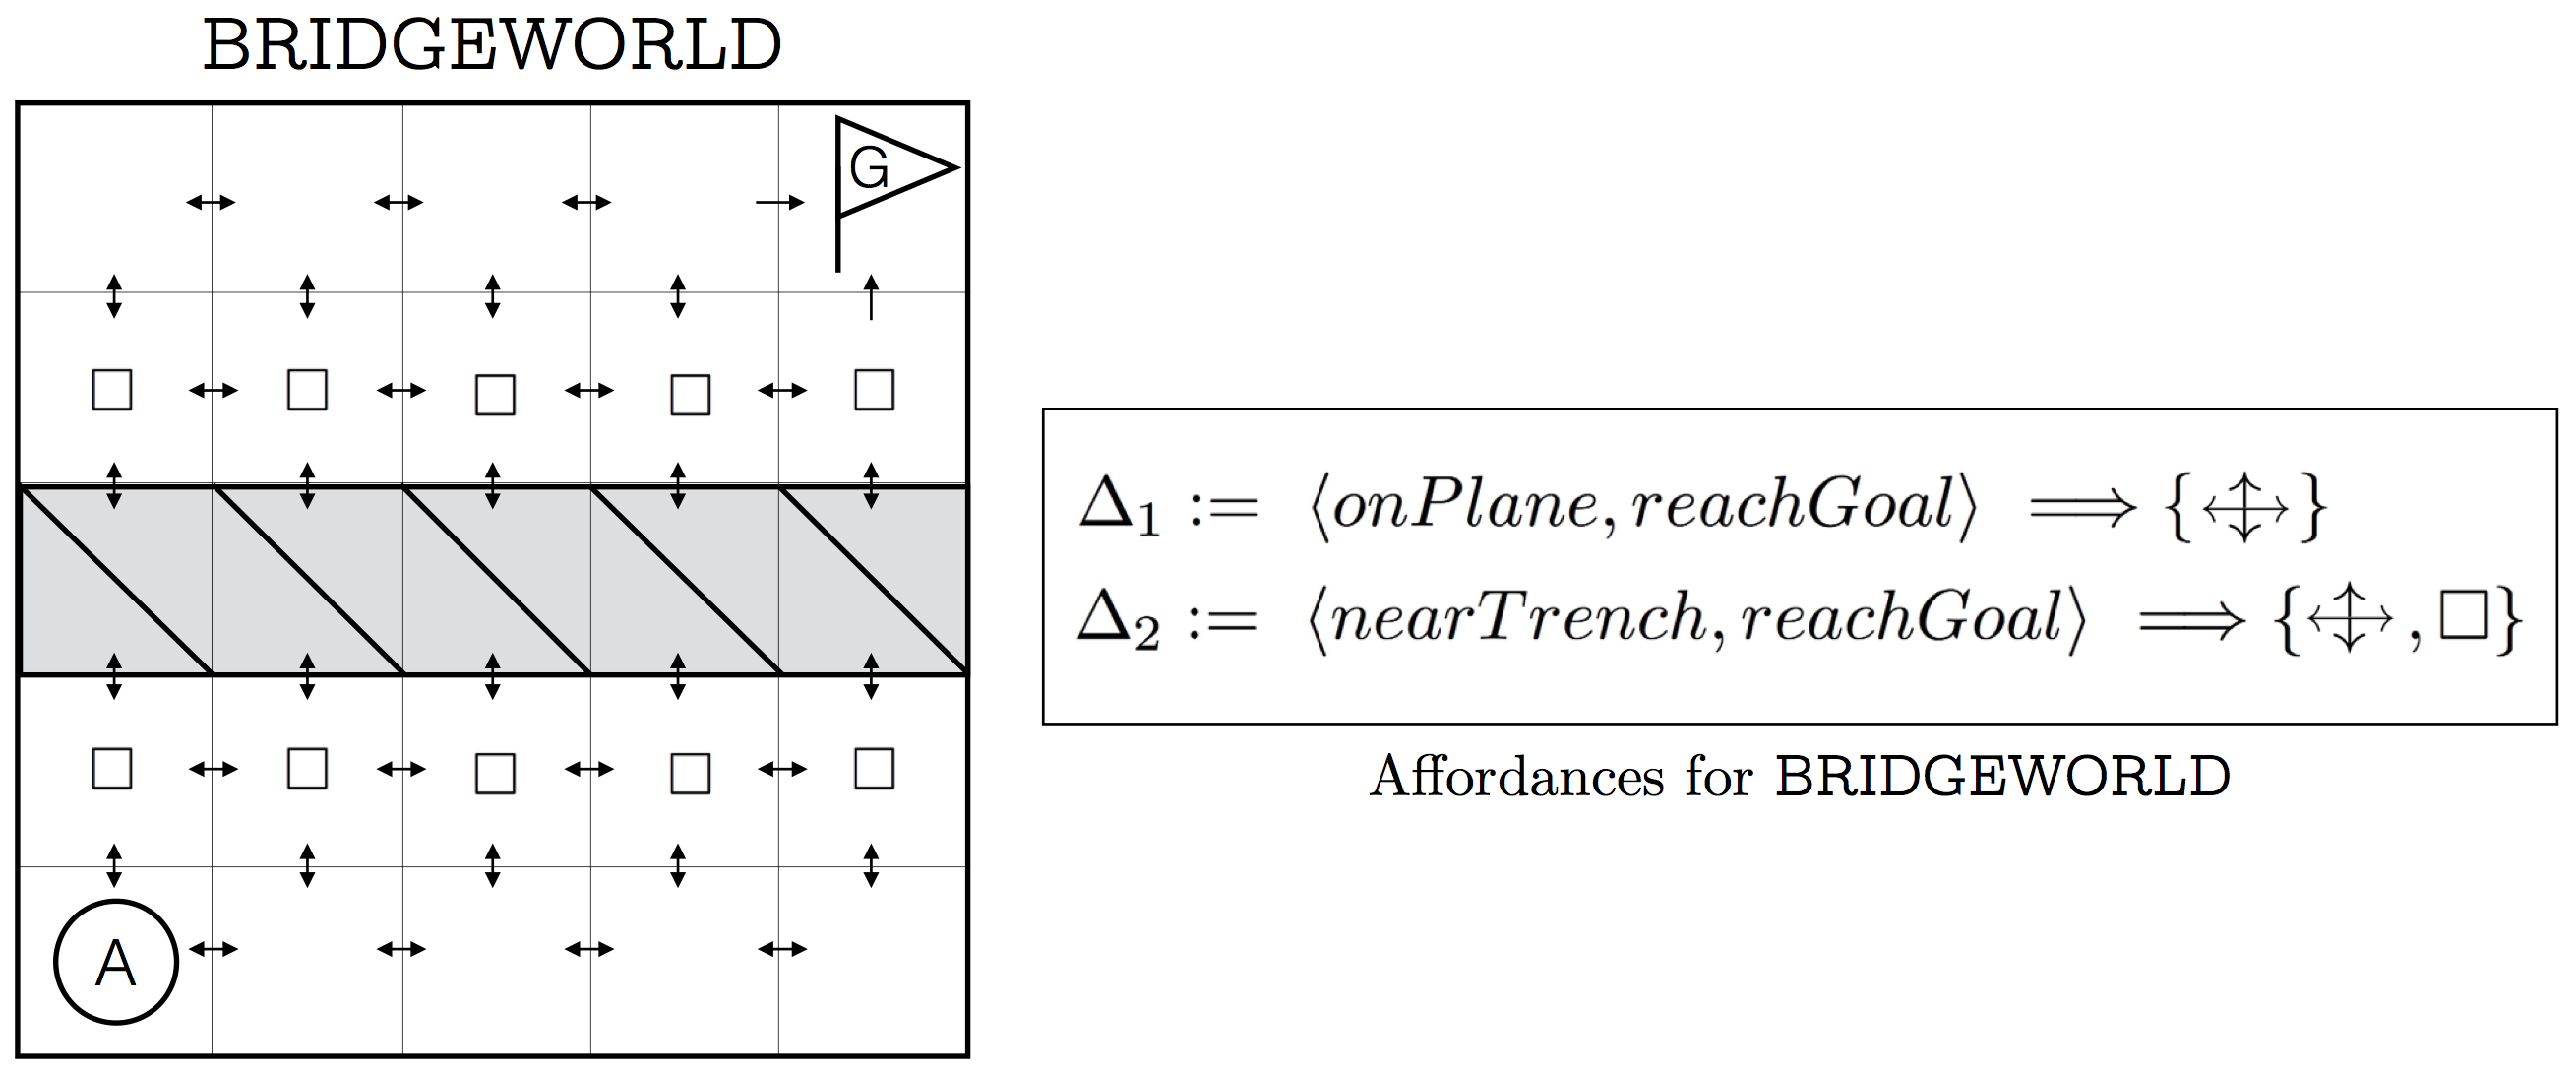
\includegraphics[scale = 0.18]{figures/bridgeworld_aff.png}
\caption{In the above Minecraft planning problem \texttt{BRIDGEWORLD}, the agent must place a block in the trench in order to reach the goal. This problem was only solvable by the Affordance planner.\label{fig:example}}
\end{figure}

In this paper we will formalize
the notion of an affordance as a piece of planning knowledge provided
to an agent operating in a Markov Decision Process
(MDP)~\citep{kaelbling99}.  We demonstrate that, like an option or
macro-action, an affordance provides additional information to the
agent, enabling more efficient planning.  However, unlike previous
approaches, an affordance enables more significant speedups by
reducing the size and branching-factor of the search space, enabling
an agent to focus its search on the most relevant part of the problem
at hand.  This approach means that a {\em single} set of affordances
provides general domain knowledge, becoming relevant just when the
agent reasons that it needs to pursue a particular subgoal.  Furthermore,
Affordances are not specific to a particular state-space nor problem-type, and thus, provide
the agent with transferrable knowledge that is effective in a wide variety of
domains and problems, unlike other approaches.


\begin{figure}
\centering
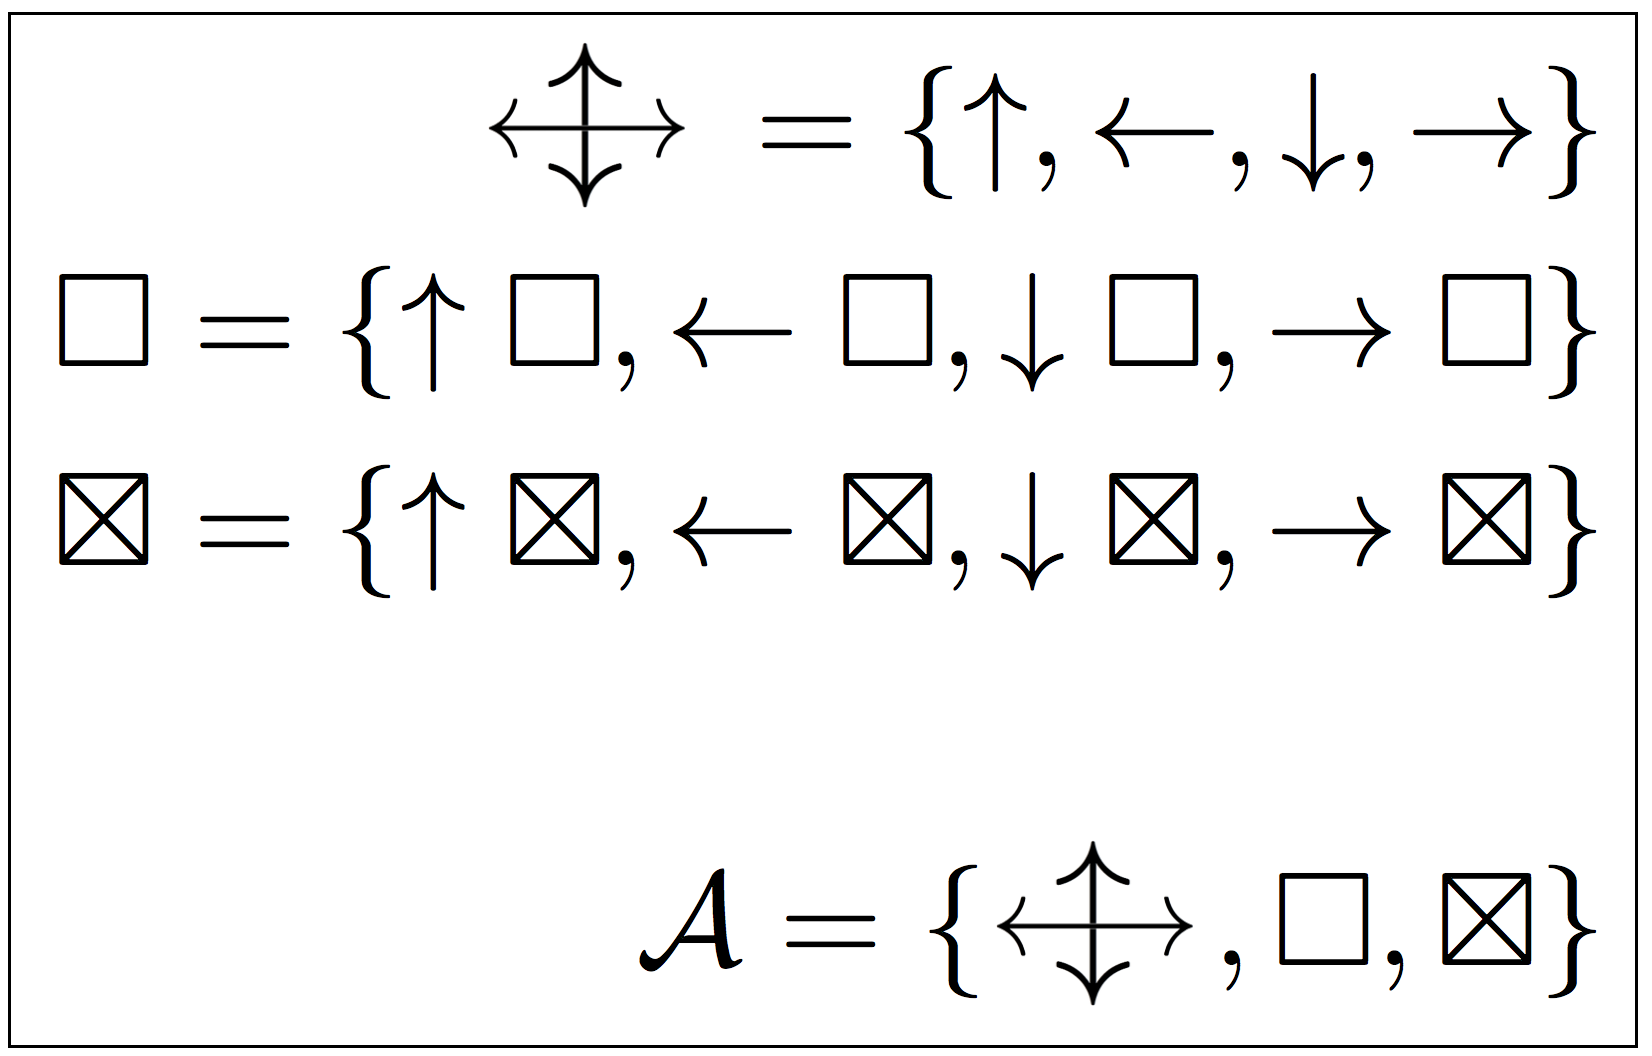
\includegraphics[scale = 0.12]{figures/mc_action_set.png}
\caption{The agent's set of actions in the Minecraft domain ($\square$ is the set of placement actions, $\boxtimes$ is the set of destruction actions)\label{fig:example}}
\end{figure}

\section{BACKGROUND}

\subsection{OOMDP}

The Object Oriented Markov Decision Process (OO-MDP) ~\citep{diuk08} is an extension of the classic Markov Decision Process (MDP). Recall that a finite MDP is a five-tuple: $\langle \mathcal{S}, \mathcal{A}, \mathcal{T}, \mathcal{R}, \gamma \rangle$, where $\mathcal{S}$ is a state-space, $\mathcal{A}$ is the agent's set of actions, $\mathcal{T}$ denotes $\mathcal{T}[s' \mid s,a]$, the transition probability of an agent applying action $a \in \mathcal{A}$ in state $s \in \mathcal{S}$ and arriving in $s' \in \mathcal{S}$, and $\mathcal{R}(s,a)$ denotes the reward at $s$ when action $a$ is applied, and $\gamma$ is a discount factor. The OO-MDP changes the underlying representation of the state space $S$ so that worlds are more general. Planning with an OO-MDP involves running Value Iteration to determine a policy.

In practice, basic Value Iteration scales very poorly, either as the state space grows, or the action set grows. This is because the state-action space, depending on the domain, grows exponentially w.r.t the number of ways that the agent can change the environment. This is ameliorated slightly by introducing the OO-MDP, but it still fails in just about all of the planning scenarios we introduce here. On \texttt{BRIDGEWORLD}, the planner was incapable of enumerating the state space prior to filling up a 2Gb Java heapspace, presented with a single block and minimal action set (it could only place blocks in front of it, and could not destroy blocks) and thus, failed outright.

The reason for this failure is that in classical Value Iteration, the agent tries to explore all states that result from applying every action in every state - this is downright silly, as in \texttt{BRIDGEWORLD}, the agent will inevitably end up in the corner of the room placing and destroying blocks. This is an especially bad tactic in the Minecraft domain, as block placement results in a combinatoric explosion of the state space. Thus, in these scenarios, our Affordance planner has a substantial advantage on classic Value Iteration. These weaknesses are well known ~\citep{grounds}, and have resulted in attempts to make planning more practical in domains of a larger scale.

% Value Iteration
% More details on OO-MDP

\begin{figure}
\centering
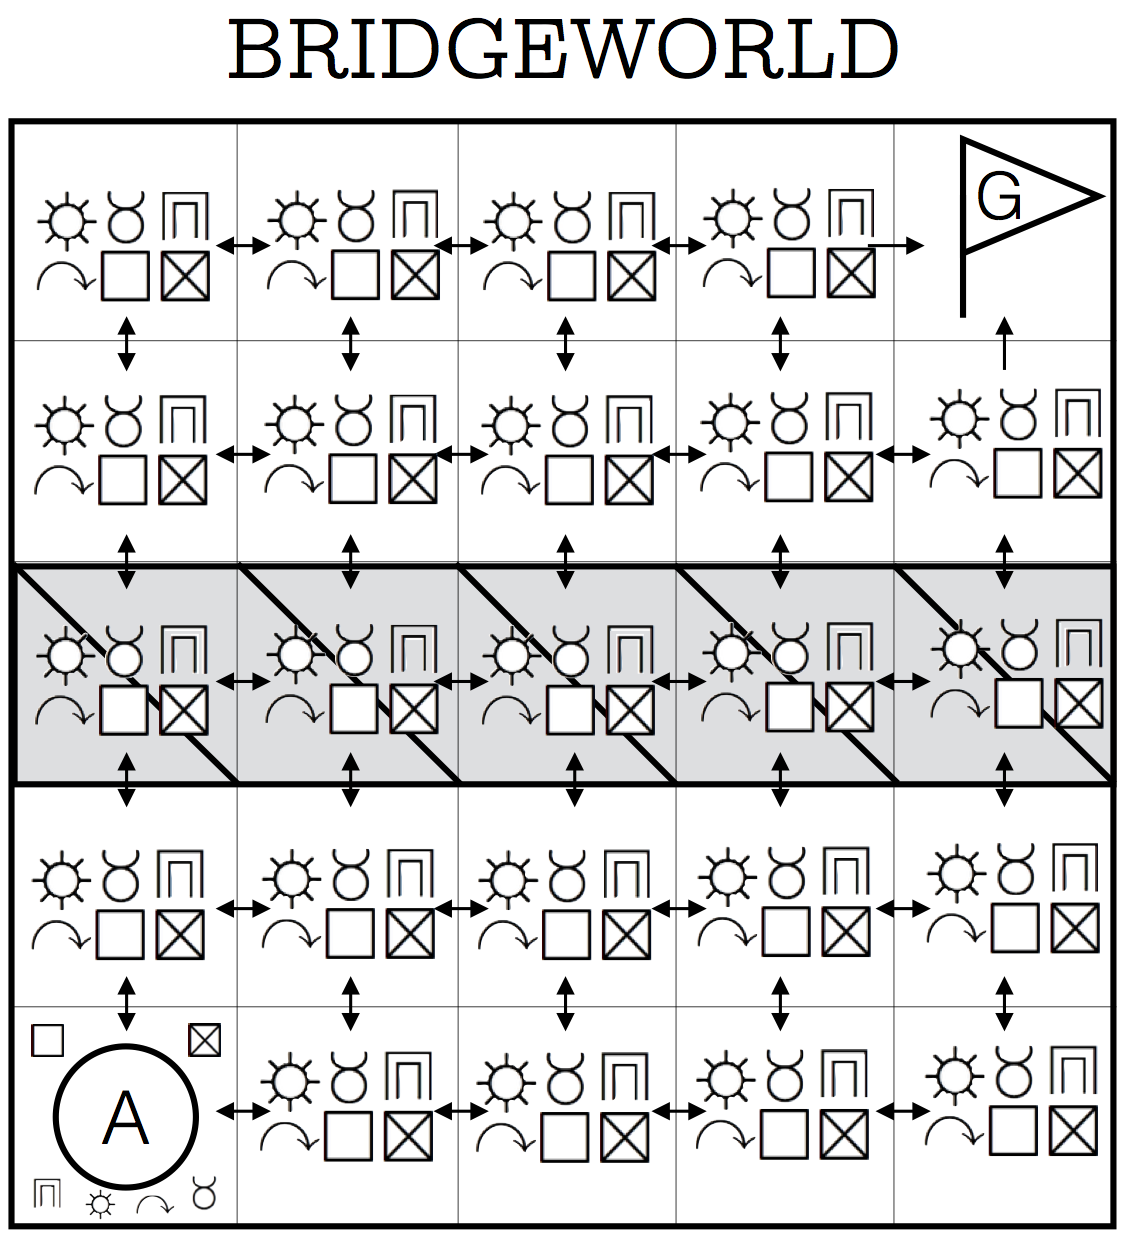
\includegraphics[scale = 0.2]{figures/bridgeworld_vi.png}
\caption{Reachability while running VI}
\end{figure}

\subsection{SUBGOALS}
% % Intuition
Subgoal planning leverages the intuition that certain goals in planning domains may only be brought about if certain preconditions are first satisfied. For instance, in the Minecraft domain, one must be in possession of grain in order to bake bread. In Branavan et. al~\citep{branavan}, they explore learning subgoals from the Minecraft wiki and applying them in order to plan through a variety of problems in Minecraft.

% Formalism
Formally, in subgoal planning, the agent is set of subgoals, where each subgoal is a pair of predicates:

\[ 
SG = \langle x_k, x_l \rangle
\]

where $x_l$ is the effect of some action sequence performed on a state in which $x_k$ is true. Thus, subgoal planning requires that we perform high-level planning in subgoal space, and low-level planning to get from subgoal to subgoal.

%Pseudocode of algorithm

In the case of \texttt{BRIDGEWORLD}, we might consider placing a block somewhere along the trench to be a subgoal. Then, we run Value Iteration to get from the agent's starting location to the point at which we've placed a block in the trench, stop, and run Value Iteration again from the first subgoal to the finish. There are a few problems with this approach, however.

% Maybe consider inserting Branavan's chart (or similar), or discuss how the search in subgoal space works?

{\bf Problem 1: Loss of generality}  One important thing to note about subgoals that {\it are} general enough to enhance an agent's planning abilities in a wide variety of state spaces is that they propose {\it necessary} claims about the domain that the agent occupies. If the subgoals are {\it contingent} (i.e. true in some state spaces of the domain but not in others), then they can be shown to completely lose their scalability. For instance, consider the task in \texttt{BRIDGEWORLD}, in which the agent must place a block in the trench that separates the agent from the goal. The subgoal $<blockInTrench, reachGoal>$ might be a perfectly useful subgoal in \texttt{BRIDGEWORLD}, but an adversary could easily come up with thousands of worlds in which such a subgoal would completely derail the agent's planner. Thus, many subgoals do not scale beyond a particular instance of a state space. In order for subgoals to be useful, they must be necessary claims about the domain, otherwise, one can always come up with a counter world (by definition of necessary). 

{\bf Problem 2: Granular Planning} The second problem is that those that subgoals that do scale across state spaces are often not useful. For instance, the vast majority of tasks in Minecraft are not so easily broken into useful, necessary subgoals. Movement, for instance, is particularly difficult. As stated before, scalable subgoals must be necessary preconditions for a particular goal, and such preconditions are often difficult to come up with in a way that actually makes planning easier. One idea would be to create the movement subgoal that the agent is one away from the goal - this is a poor choice however, since this subgoal is hardly useful unless we repeat it (i.e. the agent is one away from the next subgoal, and so on). The result is an extremely granular and low level planning system that is no better than standard Value Iteration. If necessary preconditions existed for many goal types, then subgoal planning would be a great approach. Unfortunately, coming up with such subgoals is not an easy task, and often the best we can do is to plan at such a low level that we lose any benefit of planning over subgoals to begin with

% FIGURE OF PROBLEM 2

{\bf Problem 3: Researching the Space} The last problem with subgoal planning is that the use of subgoals actually requires that we research a huge portion of the state space. Consider the \texttt{BRIDGEWORLD} example in which the subgoal is to place a block along the trench somewhere - once we plan from the state in which a block has been placed at the trench, we research the entire first side of the trench. This problem only magnifies as you add more subgoals.

\begin{figure}
\centering
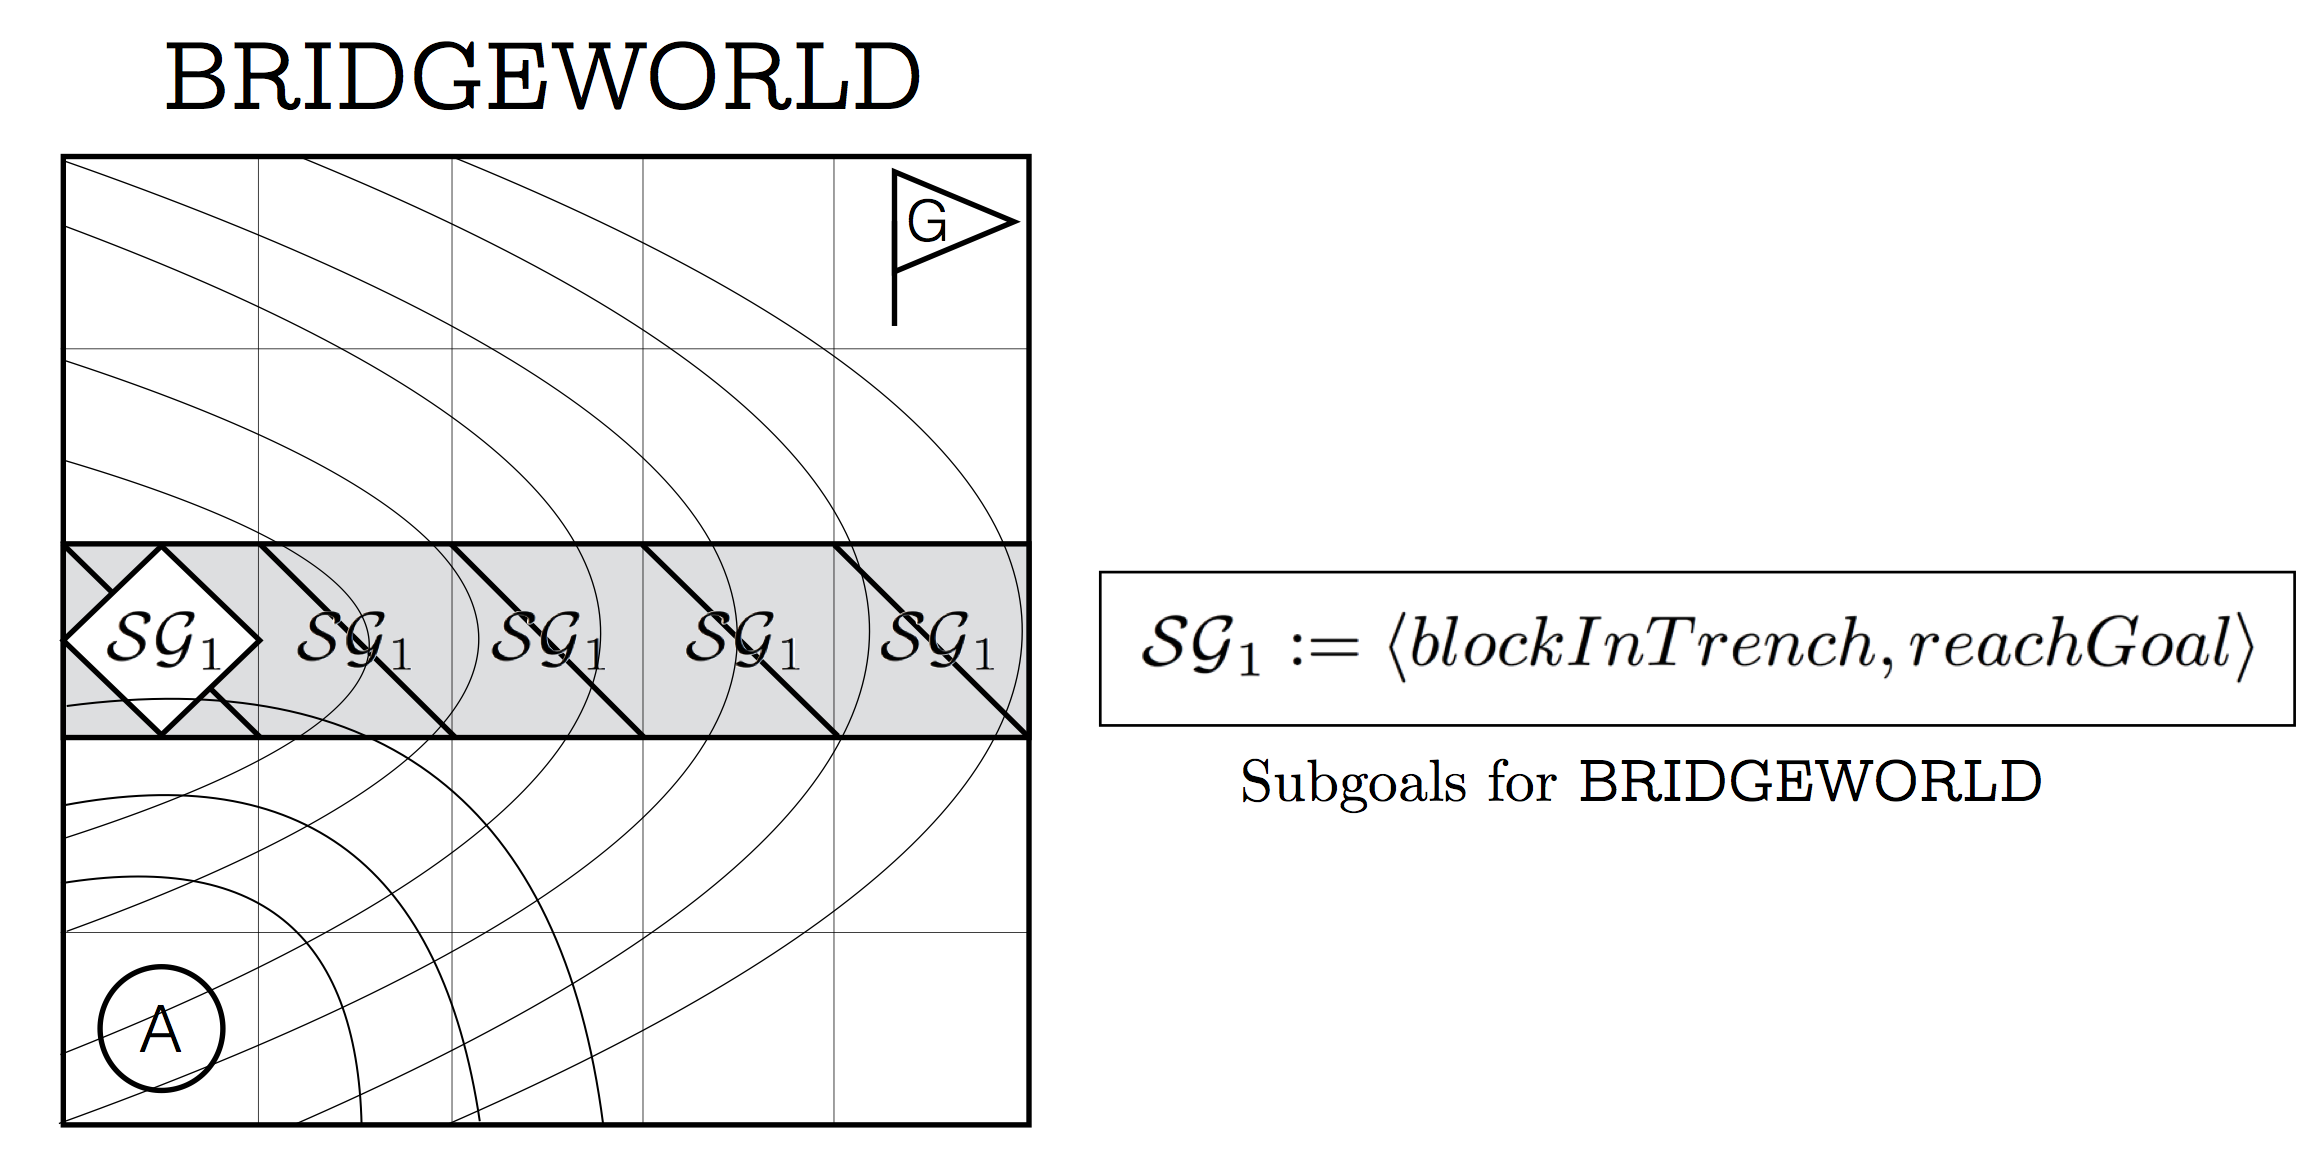
\includegraphics[scale=0.22]{figures/bridgeworld_sg.png}
\caption{The agent re-explores a large portion of the state space once it finds $\mathcal{SG}_1$. Also note that this subgoal highlights {\bf Problem 1}, in that it would be useless in many other Minecraft state spaces}
\end{figure}


A final, but less significant problem, is that Subgoal planning still requires the use of Value Iteration, which does not scale well - if there is ever a case in which planning between two subgoals is at all complex, then Subgoal planning is out of luck.

\subsection{OPTIONS}

The options framework proposes incorporating high-level policies to accomplish specific sub tasks. For instance, when an agent is near a door, the agent can engage the `door-opening-option-policy', which switches from the standard high-level planner to running a policy that is hand crafted to open doors. An option $o$ is defined as follows:

$o\ =\ \langle \pi_0, I_0, \beta_0\rangle$, where:

\begin{itemize}
\item[] $\pi_0 : (s,a) \rightarrow [0,1]$
\item[] $I_0 : s \rightarrow \{0,1\}$
\item[] $\beta_0 : s \rightarrow [0,1]$
\end{itemize}

Here, $\pi_0$ represents the {\it option policy}, $I_0$ represents a precondition, under which the option policy may initiate, and $\beta_0$ represent the post condition, which determines which states terminate the execution of the option policy.

As Konidaris and Barto point out, the classic options framework is not generalizable, as it does not enable an agent to transfer knowledge from one state space to another. Recently, Konidaris and Barto's ~\citep{konidaris} expand on the classic options framework and allow for a more portable implementation of options. Still, though, planning with options requires either that we plan in a mixed space of actions {\it and} options (which blows up the size of the search space), or requires that we plan entirely in the space of options. Additionally, providing an agent with an option policy is a difficult task for a human designer (especially if we want an optimal policy, which we do).

\subsection{MACROACTIONS}

\[
\boxed{\text{Running Example}}
\]

\section{AFFORDANCES}

%% Formalism
Formally, an Affordance is defined as \vspace{1 mm} \\
{\it Aff} $ =\ \langle p,g\rangle\ \longrightarrow \alpha$, where:

\begin{itemize}
\item[] $\alpha \subseteq \mathcal{A}$
\item[] $p : s \longrightarrow \{$0$, 1\}$
\item[] $g : s \longrightarrow \{$0$,1\}$
\end{itemize}

Where $\alpha$ is a subset of the agent's given set of actions $\mathcal{A}$, $p$ is a {\it precondition} that is a predicate over states, and $g$ is a {\it goal} or {\it subgoal} that is also a predicate over states.

The constituents that make up an Affordance parallel those of the other planning approaches discussed in the background section.

%PseudoCode

The Affordance formalism introduced above and expanded on in this paper resolves the weaknesses of these other frameworks by limiting the complexity of the seed knowledge required of the designer, while still providing enough knowledge to limit the search space but also maintain scalability.



We should be able to prove that given a ``good" set of subgoals the agent will be able to reach one after the other with high probability. Therefore, in the case that the agent cannot reach a subgoal there is likely a better one. The agent should then prompt for a more specific subgoal that will better allow it to reach the next one.

\section{EXPERIMENTS}

We tested each planning algorithm (vanilla Value Iteration, Subgoal planning, Options, Affordance planning, Macro-action planning) on 5 distinct tasks, each with its own state space and goal-type. 

In the first set of iterations, Options, Subgoals, Macro-actions, and Affordances were all given a hand crafted set of knowledge for each individual task.

For each iteration, we measured the wall-clock time to find the goal, the percentage of the state-space explored, and the number of states that were re-explored (in the case of subgoals).

In the second round, we required that each system use one set of knowledge to solve all five planning scenarios. We ran the algorithms on the same set of tasks.

The set of tasks were inspired by those planning scenarios that the creators of each other planning system proposed.

{\bf Task One: \texttt{FLATLAND}}
% Figure or brief explanation

% Knowledge base provided for each in ROUND A

{\bf Task Two: \texttt{BRIDGEWORLD}}
% Figure or brief explanation

% Knowledge base provided for each in ROUND A

{\bf Task Three: \texttt{LIGHTWORLD}}
% Figure or brief explanation

% Knowledge base provided for each in ROUND A

{\bf Task Four: \texttt{U-WALL}}
% Figure or brief explanation

% Knowledge base provided for each in ROUND A

{\bf Task Five: \texttt{BAKE BREAD}}
% Figure or brief explanation

% Knowledge base provided for each in ROUND A

% ---- Also include the knowledge base provided for each in ROUND B, where that KB must solve all 5 tasks

\section{RESULTS}

\subsection{ROUND A:}

% We would like a table like this:
\begin{figure}
\begin{tabular}{ l || c | c | c | c }
  & Affordances & Options & Subgoals & VI \\
  \hline
  {\bf T1} & 1 & 1 & 0 & 0  \\
  {\bf T2} & 1 & 1 & 0 & 1 \\
  {\bf T3} & 1 & 1 & 1 & 0 \\
  {\bf T4} & 1 & 1 & 0 & 0 \\
  {\bf T5} & 1 & 1 & 0 & 0 \\
\end{tabular}
\caption{Results of running each algorithm ten times in Round A on each of the five tasks described above . Units are in 
wall-clock time.}
\end{figure}


\subsection{ROUND B:}

% We would like a table like this:
\begin{figure}
\begin{tabular}{ l || c | c | c | c }
  & Affordances & Options & Subgoals & VI \\
  \hline
  {\bf T1} & 1 & 1 & 0 & 0  \\
  {\bf T2} & 1 & 1 & 0 & 1 \\
  {\bf T3} & 1 & 1 & 1 & 0 \\
  {\bf T4} & 1 & 1 & 0 & 0 \\
  {\bf T5} & 1 & 1 & 0 & 0 \\
\end{tabular}
\caption{Results of running each algorithm ten times in Round B on each of the five tasks described above . Units are in 
wall-clock time.}
\end{figure}
% As well as some charts indicating search space size, #cycles, etc..

\section{CONCLUSION}

% Recap contribution paragraph

% Future work: Learning, making result of each affordance probabilistic to prune away even more.


\bibliographystyle{plainnat}
\bibliography{main}  


\end{document}
